\section{Introduction}
\label{sec:intro}

% Key/value stores remain a fundamental building block of modern
% scale-out service architectures.  Recent trends in primary storage
% technologies, however, are pushing operators to consider ever-more
% disaggregated designs for their in-memory storage systems.
% Concretely, increases in CPU core counts coupled with stagnating DRAM
% density has led to an increased interest in remote memory tiers, where
% some portion of memory is connected to the server over a network.
% Moreover, once disaggregated, memory can be pooled to achieve greater
% cost and power efficiencies.  The challenge facing fully disaggregated
% memory pools, however, is managing concurrent updates in the face of
% client failures and high access latencies.

% While cache-coherent technologies like CXL are beginning to
% become available, RDMA remains the commodity option for
% large-scale in-memory key/value stores.
% Many prior RDMA-based systems opt for a partially
% disaggregated model, in which a CPU core is collocated with
% remote memory to provide the needed
% serialization~\cite{erpc,herd,pilaf,cell,clover,sherman}.
% Fully disaggregated systems rely upon one-sided RDMA atomic
% operations (e.g., compare-and-swap) to resolve data
% races~\cite{rolex,fusee,race} which constrains their design.
% Specifically, RDMA atomic operations can act upon 64 contiguous bits
% of memory at a time at most, leading to implementations that employ
% multi-stage datastructures to support practical key and value sizes.

% In general, existing systems rely upon a high-performance index
% structure to localize key operations and maintain values separately,
% necessitating multiple RDMA operations and network round trips even in
% the absence of contention.  Moreover, given the dominance of
% read-heavy workloads~\cite{rocks-db-workload,facebook-memcached}, most
% systems eschew locks in favor of optimistic update approaches that can
% lead to poor performance under contention.
% In this work we design an index datastructure tailored for the
% constraints of current RDMA hardware.  Specifically, we
% facilitate lock-based updates by decreasing the number of round
% trips required to acquire locks and perform mutating operations.

Disaggregated architectures aim to improve scalability and utilization
by pooling network-attached
resources~\cite{dredbox,firebox,blade-server,legoos}.  In theory,
pooling reduces per-machine fragmentation and stranding by exposing
resources over the network. Collectively, disaggregated resources can
be provisioned for the sum-of-peak workloads rather than the
peak-of-sums~\cite{dsnf,supernic}. Stagnating DRAM
densities are driving interest in primary storage pooling, but
performant, general-purpose far-memory tiers remain
elusive~\cite{fastswap,3po,kona,infiniswap,hydra,leap,legoos,dilos} as
even the fastest rack-scale networks have access
latencies that are an order-of-magnitude slower than local memory.
%Current RDMA technologies have access latencies that are 20 times that of local
%DRAM
(e.g., RDMA latency is approximately 1~{\textmu}s versus DRAM's
50~ns)~\cite{clover}.

% High access latencies are particularly challenging for systems that seek to support shared
% read/write workloads due to the need to synchronize updates, as coordination costs do not decrease
% as link bandwidths improve, causing them to become the bottleneck to system performance.
% %Sharing disaggregated memory is fundamentally hard because cost of synchronization is high.
% As a result, most existing far-memory systems choose to statically partition memory and optimize
% performance through a variety of client-local techniques~\cite{kona,mira,aifm,trackfm,carbink}.
% %(cache policy, compilers, pointer analysis
% To date, the most promising approach to deliver shared access to pooled remote memory is to expose a
% key/value store (KVS) interface that provides coherent read/write
% semantics~\cite{rolex,smart,ditto,fusee,clover,sherman,ford}.


As a result, most existing far-memory systems~\cite{kona,mira,aifm,trackfm,carbink} choose to statically partition remote memory to avoid the multiple round trips required to 
synchronize shared updates.
%\footnote{lock/unlock or optimistic concurrency} requires multiple round
%trips per operation at 20x the cost
%%
%We argue that, 
While challenging to achieve, memory sharing is
critical to making remote memory pooling practical as it can
improve utilization---the entire point of memory
disaggregation.  To date, the most promising approach to delivering
shared access to pooled remote memory is to expose a key/value store
(KVS) interface that provides coherent read/write
semantics~\cite{rolex,smart,ditto,fusee,clover,sherman,ford}.  Yet,
most performant KVS systems employ two-sided RDMA operations which rely upon
memory-side CPUs to manage locks and execute critical
sections~\cite{memc3,cuckoo-improvements,pilaf,cell}, reducing their
potential savings.

To fully unlock the potential of memory disaggregation, we propose a
design where compute and memory are entirely separate. In our fully
disaggregated model, a KVS must implement a client-side serialization protocol
implemented entirely in one-sided RDMA operations (i.e., read, write, and atomic
updates).  Maintaining a coherent memory model is the core challenge in
designing such systems. Existing KVS's with ordered keys
% When building a fully disaggregated KVS, a critical design decision is
% selecting an approach to managing race conditions in the absence of
% server-side CPUs that are powerful enough to mediate client requests.  The
% core challenging in designing a disaggregated KVS is efficient serialization.
% Memory disaggregation assumes that machines housing pooled DRAM do not have
% CPUs powerful enough to service requests.  Existing systems require Thus,
% clients must implement their own serialization protocols. These protocols use
% Commodity RDMA devices provide one-sided verbs that enable client-only
% synchronization, and existing systems carefully coordinate reads, writes, and
% atomic operations to maximize performance while delivering coherent access.
% Systems that implement datastructures with ordered keys 
(e.g., BTrees \& Radix Trees) rely upon locking schemes~\cite{smart,sherman},
while those that provide unordered access favor lock-free
techniques~\cite{rolex,ditto,fusee,clover} to decrease read latency while
avoiding the RDMA hardware bottlenecks and complex failure scenarios that can
arise with locks.  The trade-off, however, is that lock-free approaches perform
worse as write intensity increases.
%Indeed, prior lock-based systems assume that clients are co-located---and can
%therefore combine writes---and do not tolerate client
%failure~\cite{sherman,smart}.

In this work we present RCuckoo, a system that uses lock-based synchronization
on commodity RDMA hardware to out-perform existing key/value stores across a
wide range of workload mixes.
%It is
%well known that opportunistic lock-free approaches perform poorly
%under high levels of contention, and we show that it is possible to
%design a lock-based system that not only delivers high throughput for
%read/write workloads, but out-performs existing systems on read-only
%workloads as well.
Critically, locks enable the use of cuckoo hashing~\cite{cuckoo}, a
well-established, high-performance datastructure for key/value stores.
Locks also support in-lining small values in the hash table,
%cuckoo
%hashing requires only one round trip to service
%uncontested read requests yielding
%By using locks we can enable inlined operations on KVS indexes which can
%result in
delivering
significantly higher throughput on common mixed read/write workloads.
Further, our fine-grained locks and careful protocol design reduce
lock hold times during updates to two round trips in the common
case, and we avoid known hardware bottlenecks with RDMA atomic
operations by crafting a lock table small enough to be stored entirely
on NIC-based memory.  Finally, lease-based lock acquisition
delivers correct, high-throughput performance even in the
face of client failures with held locks.

RCuckoo's efficient locking is made possible by a \emph{dependent
hashing} algorithm that makes spatial locality a tunable parameter.
Cuckoo hashing works by deterministically computing two potential hash
locations---primary and secondary---for any key; collisions are
resolved by relocating the existing entry in a key's primary location
to the existing key's secondary location, and so on down what is known
as a cuckoo path.  Traditionally, a key's two potential locations are
drawn independently at random, defeating any locality-based
optimizations.  By controlling the distance between a key's
locations---and therefore the span of a potential cuckoo path---we
probabilistically bound the range of memory that must be locked, and,
relatedly, the number of locks that a client must acquire.

%Concretely, by controlling how physically far apart alternate locations for a

%Locality is the linchpin of our design as it enables us to efficiently determine
%the ranges of memory each operation needs and acquire the right locks.



\begin{figure*}[t]
    \centering
    \newcommand{\subfigwidth}{0.32\linewidth}
    \begin{subfigure}{\subfigwidth}
        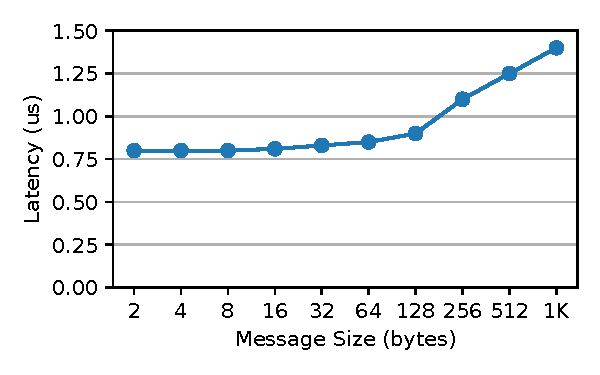
\includegraphics[width=0.99\linewidth]{fig/rdma_latency.pdf}
    \end{subfigure}
    \begin{subfigure}{\subfigwidth}
        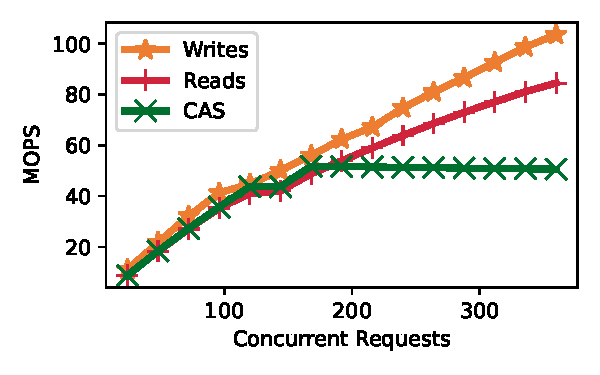
\includegraphics[width=0.99\linewidth]{fig/rdma_concur.pdf}
        % \label{fig:optimistic_failures}
        % \caption{}
    \end{subfigure}
    % \begin{subfigure}{\subfigwidth}
    %   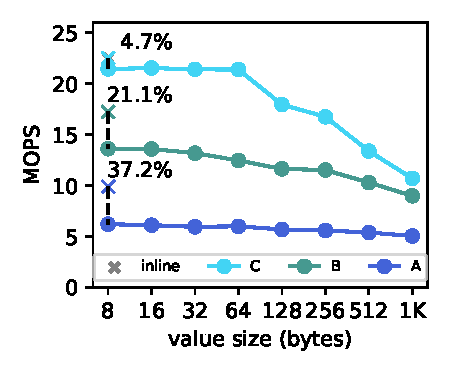
\includegraphics[width=0.99\linewidth]{fig/extent.pdf}
    % \end{subfigure}
    \begin{subfigure}{\subfigwidth}
        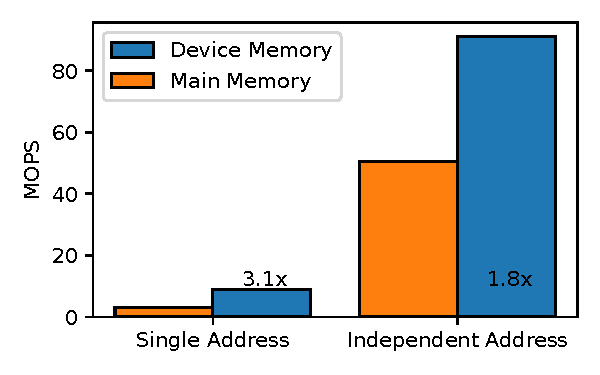
\includegraphics[width=0.99\linewidth]{fig/rdma_cas_throughput.pdf}
    \end{subfigure}
    \vspace{-1em}
    \caption{Basic RDMA performance on our testbed.
    % \textbf{(a)} (64-bit) operations per second;
    \textbf{(a)} Read latency as a function of message size~\cite{rdma-latency}.
    \textbf{(b)} Operation throughput as a function of offered load.
    \textbf{(c)} Atomic compare-and-swap performance on device and main memory.
    }
    \label{fig:rdma-benchmarks}
\vskip -1em
\end{figure*}

Combined with aggressive
batching of RDMA operations, RCuckoo's spatial locality limits the
number of round trips required for all table operations.  In the
common case, reads execute in one (for small values) or two round
trips, uncontested updates and deletes require two round trips, and
the median insert operation involves only two round trips---although
the expected number increases as the table fills and cuckoo paths
grow.  On our testbed, RCuckoo delivers comparable or higher
performance on small values across the standard set of YCSB benchmarks
than all of the existing disaggregated key/value stores we consider.
Concretely, with 320 clients RCuckoo delivers up to a 2.5$\times$
throughput improvement on read-intensive (YCSB-B) workloads and up to
7.1$\times$ their throughput on write-intensive (YCSB-A) workloads.
Moreover, RCuckoo's performance remains high despite 100s of clients
failing per second.
